\chapter{Le développement de jeux vidéos}
 \textcolor{red}{Trouver une manière d'introduire le chapitre}
 
\section{Les étapes de création}
%Conférence Ubisoft a l'UQAM
Les étapes de développement d'un jeu vidéo ne sont pas immuables et dépendent de l'entreprise, du domaine d'activité ou des collaborateurs impliqués dans le projet. La liste suivante est non exhaustive et a été présentée par Mathieu Nayrolles lors d’un séminaire au LATECE (Laboratoire derecherche sur les technologies du commerce électronique) de l’UQAM.
\begin{figure}[H]
    \centering
    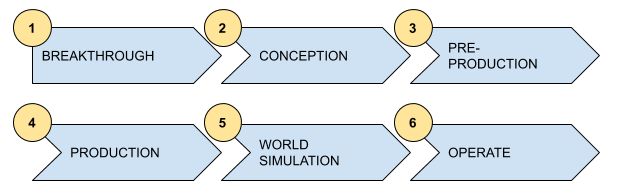
\includegraphics[width=14cm]{10_img/production_stages.png} 
    \caption{Étapes de création d'un jeu vidéo}
\end{figure}
\subsection{Breakthrough}
Une étape de Breakthrough permet de réunir une équipe afin d'effectuer des recherches et explorations sur des nouvelles mécaniques ou des nouvelles technologies afin de créer du nouveau contenu. Cette étape est optionnelle dans un projet.
Par exemple :
\begin{itemize}
    \item Une percée technologique. Ex : Google lance Stavia une plateforme en ligne de jeux vidéos sous forme de catalogue et jouable à 100\% en ligne sans installation en local
    \item Une percée de Gameplay. Ex : naissance du mode Battle Royale
\end{itemize}

\subsection{Conception}
Un document de concept est prototypé afin de définir l'environnement, la faisabilité et l'intérêt commercial du jeu. C'est durant cette étape que les game designer définissent et précisent l'univers, les mécaniques et le déroulement du jeu vidéo en question. Cette étape est majoritairement gérée par les Game Designers appuyés par les équipes des autres corps de métier. Dans des projets à financements externes cette étape est cruciale. Elle permettra de présenter le projet à un studio avec une première maquette permettant de présenter les fondements du jeu.

\subsection{Pre-production}
Durant cette étape des prototypes sont développés afin de créer une version minimale du jeu. Ces prototypes permettent d'avoir un aperçu jouable des concepts définis durant la phase précédente. Un prototype est une coupe verticale de tout le système qui permet de valider ou redéfinir les concepts. Une fois le design bien définit, le prototype au plus proche de ce que donnerait le jeu final et la faisabilité du projet confirmée, il est alors possible de rechercher les financements et les ressources nécessaires à la production. Cette étape est gérée par tous les corps de métier dans un studio de développement, tous les aspects du jeu devant être représentés afin de montrer tout le potentiel du prototype.

\subsection{Production}
Une fois les fonds levés et les ressources humaines attitrées au projet, il est alors possible de procéder à la production du jeu vidéo. Tous les corps de métier sont alors représentés et le jeu est développé sous tous ses aspects et dans son intégralité. La plupart du temps le développement est découpé en plusieurs itérations. Chacune d'entre elles permet de vérifier que le jeu respecte bien les concepts définis plus tôt. C'est également à ce moment là que les dernières modifications sont apportées aux concepts afin qu'ils respectent la vision du Game Designer et génèrent la bonne expérience. Dans le cas ou le projet rencontre des contraintes supplémentaires (temps, argent, plateforme...) les concepts peuvent également être revus en conséquence. Généralement durant cette étape le marketing et la publicité autour du jeu commencent à prendre place afin de prévenir le public et d'estimer l'impact que peut avoir le jeu.

\subsection{Simulation}
Lors de la simulation tous les éléments du jeu sont testés et passés au crible. On vérifie que les éléments de jeu soient correctement modélisés, que les sons correspondent bien aux éléments, que les personnages correspondent à ceux décris dans les documents de conception... Plusieurs questions se posent à ce moment là. 
\begin{itemize}
    \item Est-ce que les éléments interagissent bien entre eux ?
    \item Est-ce que l'univers de jeu est cohérent de bout en bout ?
    \item Est-ce que le gameplay est fluide et intuitif ?
    \item Est-ce que l'environnement de jeu est réellement comme le décrit le game designer ?
    \item Est-ce que la bande sonore ou la modélisation graphique génère bien l'émotion attendue chez le joueur ?
\end{itemize}

\subsection{Distribution et fonctionnement}
Le jeu est maintenant produit et commercialisé. Une quantité importante de données est ainsi générée. Des bugs peuvent être remontés et corrigés dans des cas de figure particuliers ou inédits non couverts par l'étape de World Simulation. Des ajustements mineurs peuvent être fais en fonction des besoins ou des demandes des joueurs. Le jeu prend alors toute sa dimension et toute sa vie à travers les joueurs.

\subsection{Nouveau contenu}
Une fois le jeu bien en place et les étapes de corrections et ajustements passées, il est possible alors d'intégrer du nouveau contenu au jeu en repassant par les étapes précédentes. Ce nouveau contenu est généralement intégré au sous forme de mises à jours (gratuites) ou de \gls{dlc} (payantes).



\section{Exploitation et exploration}
Il est nécessaire pour les studios de développement de jeux vidéos de trouver le bon équilibre entre exploitation et exploration. Le but étant d'offrir aux clients des articles de qualité et attractifs. Cet équilibre est précaire et il est difficile pour un studio de développement d'investir sur les deux domaines à la fois. Dans leur article, Parmentier et al \cite{ParmentierGuy2009Iecd} explorent la capacité des studios à concilier ces deux activités. Ils présentent les enjeux de chacune d'entre elles et leur importance dans le domaine.

\subsection{Exploitation}
L'exploitation dans le développement de jeux vidéos est une part importante du travail d'un studio de développement. De nombreux jeux vidéos récents sont basés sur de l'exploitation de jeux précédents, autant au niveau du gameplay qu'au niveau des concepts fondamentaux de jeux précédents. C'est le cas de grosses productions de franchises comme les jeux de EA sports (FIFA, NHL, NBA Live, Madden), les jeux d'action role-play de FromSoftware (série des Dark Souls), les jeux d'action aventure de Rockstar (série des GTA) ou les jeux de simulation de Maxi/EA Games (série les Sims). Le travail d'exploitation consiste à produire une suite ou un nouveau jeu en utilisant des technologies (moteur, plateformes, etc) ou un gameplay déjà existant afin de recréer un jeu ou produire du contenu additionnel. Ceci peut être fait dans un but de fidéliser une clientèle déjà existante en ajoutant du contenu additionnel à un jeu, à offrir une expérience similaire avec des technologie plus récentes (ex : FIFA) ou à offrir une suite à un jeu ayant déjà connu du succès (ex : Dark Souls).

\subsection{Exploration}
L'innovation dans le monde du jeux vidéos est essentielle au développement de nouveaux concepts de gameplay mais également de nouvelles technologies. La nouveauté est un enjeu essentiel afin d'attirer toujours plus de joueurs. L'investissement dans l'exploration est donc très important pour un studio de développement. De la recherche de nouveaux concepts de jeux, de nouveaux types de gameplay, de nouvelles technologies à intégrer ou de la création de nouveaux moteurs de jeux, l'exploration est devenu un facteur essentiel au domaine du jeu vidéo et à son expansion.



\section{Les moteurs de jeux}
Un moteur de jeu (Game engine) est le plus souvent une suite logicielle contenant un framework de mécaniques de jeu permettant d'accélérer le développement d'un jeu vidéo. Il peut inclure une ou plusieures facettes du développement du jeu allant de la physique, aux graphismes, aux sons, aux calculs, à la gestion des périphériques d'entrée/sortie jusqu'à la gestion automatique de l'intelligence artificielle. Voici une liste des moteurs de jeu les plus connus accompagnés des jeux qui en font usage : 
\begin{itemize}
    \item Unreal Engine \cite{UnrealEngine} développé par Epic Games : Fortnite, Outlast 2, Dragon Ball Fighter Z, Days Gone.
    \item Unity Engine \cite{UnityEngine} développé par Unity Technologies : 7 Days to Die, Cuphead, Ori and the Blind Forest, Pokemon Go.
    \item CryEngine \cite{CryEngine} développé par Crytek : Far Cry, Crysis 3, Deceit, Mavericks.
    \item Frostbite \cite{FrostbiteEngine} développé par Dice (EA) : Battlefield V, Anthem, FIFA, Need for Speed.
\end{itemize}

Chaque moteur de jeu présente des avantages et des inconvénients en fonction du type de jeu que l'on souhaite développer. Certains moteurs sont axés sur un type de jeu ou une plateforme en particulier afin d'être plus efficaces. L'innovation dans les moteurs de jeu est essentielle au développement de nouveaux jeux vidéos. C'est avec ces outils qu'il est possible de développer des jeux vidéos. Un moteur de jeu plus récent pourra intégrer des éléments plus récents de l'innovation comme des graphismes plus réalistes ou détaillés ainsi que des intelligences artificielles plus évoluées.

\section{Les types de Gameplay}
L'exploration peut également consister en la création d'un nouveau mécanisme de gameplay. Ce genre d'innovation est plus facilement repérable par le joueur et plus marquante concernant l'expérience de jeu. Voici une liste non exhaustive des principaux types de gameplay présents dans le jeu vidéo :
\begin{itemize}
    \item MMORPG (Massive Multiplayer Online Role-Playing Games) : Jeu massivement multijoueur en ligne mettant en scène un jeu de rôle avec différents objectifs à remplir : leveling, histoire principale/secondaire, développement social pour atteindre ces objectifs sous forme de guilde... (ex : World of WarCraft, Black Desert Online)
    \item Survival : le joueur doit survivre aux événements présents dans le jeu. Il peut devoir subvenir à des besoins vitaux, construire de nouveau objets, ou survivre aux autres joueurs présents (ex : Rust, Ark)
    \item Plateformes : un joueur contrôle un personnage qui se déplace dans un environnement de plateformes et doit avancer tout au long du niveau pour le finir (ex : Mario, Donkey Kong)
    \item Simulation de vie : Le joueur simule un environnement de vie plus ou moins réaliste en fonction des objectifs du jeu. La simulation peut s'appliquer à un personnage ou à une ville entière. (ex : Les Sims, SimCity)
    \item FPS (First Personnal Shooter) : le joueur est seul ou en équipe et doit battre les ennemis (IA ou autres joueurs) à l'aide d'armes et d'équipements de combat (ex : Call of Duty, Halo)
    \item Beat-em up : Le joueur fait face à des vagues d'ennemis toujours plus fortes (ex : Bayonnetta, God of War)
    \item RTS (Real Time Strategy) : Des joueurs se font fasse dans un jeu ou la gestion d'économie, de troupes et de population est omniprésente afin de battre les autres (Age of Empire, Starcraft)
    \item 4x (explore, expand, exploit and exterminate) : proche du RTS ce type de gameplay se base sur une gestion pointue de ressources et de population afin de pouvoir battre les autres joueurs sous différents aspects et avec différents objectifs de victoire (population max, évolution de la société, critères fininanciers...) (ex : Civilization, Stellaris)
    \item MOBA (Multiplayer Online Battle Arena) : C'est un type de gameplay ou le jeu d'action rencontre le RTS. Plusieurs équipes de joueurs sont téléportées sur une carte, chaque joueur contrôle un personnage et les joueurs doivent détruire la base de l'équipe adverse. (ex : League of Legends, DOTA)
    \item Battle Royal : Plusieurs dizaines de joueurs sont parachutés sur une carte ou ils trouvent des armes et doivent s'entretuer. le dernier vivant est déclaré vainqueur. (ex : Fortnite, PUBG)
\end{itemize}

Les types de gameplay évoluent beaucoup. De nouveaux gameplays apparaissent grâce aux recherches exploratoires. Certains modes de jeux à succès deviennent des catégories à part entière. Il est possible de combiner plusieurs modes de jeu afin de créer une nouvelle expérience. Ces types de gameplay sont classifiés en fonction du type de monde, des objectifs de jeu, des actions nécessaires... Dans l'article de Haitz et Law \cite{HeintzStephanie2015TGGM}, les auteurs mettent en place une cartographie des genres afin de classifier les différents types de jeux en se basant sur des caractéristiques précises des jeux et de leur gameplay. Cependant il est difficile d'arriver à classifier tous les jeux tellement les genres sont nombreux et entrecoupés. C'est pour cela que la plupart des jeux sont classifiés dans des catégories larges et sont différenciés par des caractéristiques différentes ensuite.



\section{Travail de recherche}
De nombreux challenges se rejoignent dans le développement de jeux vidéos et les outils et méthodes pour y parvenir sont déjà nombreux. Cependant il devient de plus en plus important dans ce secteur de chercher les méthodes possibles afin d'accélérer le développement sans pour autant impacter la qualité du contenu final. Un Game Designer se doit d'être précis et concis dans ses recherches et ses communications afin de communiquer un maximum d'informations et de pouvoir dédier plus de temps à l'exploration, à la recherche artistique et au développement d'un prototype. 

%quoi
Dans ce mémoire va être présenté \gls{gg}, un profil utilisant le \gls{uml} qui permettra d'outiller le processus de pré-conception d'un jeu vidéo, facilitant ainsi la documentation et la rédaction des documents descriptifs du jeu vidéo en cours d'élaboration.

%rapidité
Destiné à être utilisé dans les premières phases du développement, Breaktrough et Pré-conception, ce profil permet l'accélération de la documentation à travers un outil visuel représentant les mécaniques et les objets du jeu. Ceci permet de produire un prototype jouable plus rapidement.

%cohérence
L'utilisation d'un profil \gls{uml} permet d'apporter une structure précise et un cadre de travail rigoureux lors de la conception afin d'assurer la cohérence des modèles durant toute leur durée de vie.

%maintenance & modifications
Lors de sa conception un jeu vidéo est destiné à évoluer très rapidement et sa documentation se verra modifiée de nombreuses fois afin de toujours être la plus pertinente possible. \gls{uml} permet d'apporter un support visuel à cette documentation mais permet également de rendre les modifications plus faciles en accédant aux objets concernés rapidement et efficacement. 

%pérennité
Effectuer des mind mapping est un moyen simple et efficace permettant d'illustrer des idées de manière visuelle. Cependant le manque de rigueur (modifications erratiques, contenu des données incohérents, manque de structure) et les supports utilisés (feuille de papier, tableau, paper board) lors d'un travail de mind mapping n'assure pas du tout la pérennité des informations stockées. Il est en effet compliqué de modifier une photographie d'un mind mapping lors d'une réunion ayant pris place plusieurs semaines auparavant. De par sa structure imposée et précise le standard \gls{uml} permet de structurer les données, de les stocker sous un format précis et de les maintenir facilement en communiquant sur les modifications effectuées. Ceci permet un stockage beaucoup plus pérein des informations contenues dans le modèle.

%réutilisation
\gls{uml} étant un langage de modélisation largement utilisé et approuvé dans le domaine informatique, il est possible de greffer de nombreux outils permettant son utilisation, son intégration et se réutilisation dans différents cadres et sous différentes formes.

%gdd
Un modèle \gls{uml} pourra également servir de support à la rédaction d'un \gls{gdd} en organisant les mécaniques de jeu sous forme de catégories réutilisables. Le \gls{gdd} est la "bible du design" \cite{GD_foundations_pedersen} du jeu. Il permet de définir tout le contenu du jeu et toutes les informations nécessaires à son développement sur toute sa durée de vie. 

%generation de code
\gls{uml} étant reconnu comme un langage de modélisation de logiciel il peut également être possible d'utiliser les modèles créés en pré-conception afin de faciliter le développement informatique du jeu vidéo. Le modèle peut permettre de créer une structure de projet ou du pseudo code pouvant servir de "skeleton" en début de développement.



